% Options for packages loaded elsewhere
\PassOptionsToPackage{unicode}{hyperref}
\PassOptionsToPackage{hyphens}{url}
\PassOptionsToPackage{dvipsnames,svgnames,x11names}{xcolor}
%
\documentclass[
  letterpaper,
  DIV=11,
  numbers=noendperiod]{scrartcl}

\usepackage{amsmath,amssymb}
\usepackage{lmodern}
\usepackage{iftex}
\ifPDFTeX
  \usepackage[T1]{fontenc}
  \usepackage[utf8]{inputenc}
  \usepackage{textcomp} % provide euro and other symbols
\else % if luatex or xetex
  \usepackage{unicode-math}
  \defaultfontfeatures{Scale=MatchLowercase}
  \defaultfontfeatures[\rmfamily]{Ligatures=TeX,Scale=1}
\fi
% Use upquote if available, for straight quotes in verbatim environments
\IfFileExists{upquote.sty}{\usepackage{upquote}}{}
\IfFileExists{microtype.sty}{% use microtype if available
  \usepackage[]{microtype}
  \UseMicrotypeSet[protrusion]{basicmath} % disable protrusion for tt fonts
}{}
\makeatletter
\@ifundefined{KOMAClassName}{% if non-KOMA class
  \IfFileExists{parskip.sty}{%
    \usepackage{parskip}
  }{% else
    \setlength{\parindent}{0pt}
    \setlength{\parskip}{6pt plus 2pt minus 1pt}}
}{% if KOMA class
  \KOMAoptions{parskip=half}}
\makeatother
\usepackage{xcolor}
\setlength{\emergencystretch}{3em} % prevent overfull lines
\setcounter{secnumdepth}{-\maxdimen} % remove section numbering
% Make \paragraph and \subparagraph free-standing
\ifx\paragraph\undefined\else
  \let\oldparagraph\paragraph
  \renewcommand{\paragraph}[1]{\oldparagraph{#1}\mbox{}}
\fi
\ifx\subparagraph\undefined\else
  \let\oldsubparagraph\subparagraph
  \renewcommand{\subparagraph}[1]{\oldsubparagraph{#1}\mbox{}}
\fi


\providecommand{\tightlist}{%
  \setlength{\itemsep}{0pt}\setlength{\parskip}{0pt}}\usepackage{longtable,booktabs,array}
\usepackage{calc} % for calculating minipage widths
% Correct order of tables after \paragraph or \subparagraph
\usepackage{etoolbox}
\makeatletter
\patchcmd\longtable{\par}{\if@noskipsec\mbox{}\fi\par}{}{}
\makeatother
% Allow footnotes in longtable head/foot
\IfFileExists{footnotehyper.sty}{\usepackage{footnotehyper}}{\usepackage{footnote}}
\makesavenoteenv{longtable}
\usepackage{graphicx}
\makeatletter
\def\maxwidth{\ifdim\Gin@nat@width>\linewidth\linewidth\else\Gin@nat@width\fi}
\def\maxheight{\ifdim\Gin@nat@height>\textheight\textheight\else\Gin@nat@height\fi}
\makeatother
% Scale images if necessary, so that they will not overflow the page
% margins by default, and it is still possible to overwrite the defaults
% using explicit options in \includegraphics[width, height, ...]{}
\setkeys{Gin}{width=\maxwidth,height=\maxheight,keepaspectratio}
% Set default figure placement to htbp
\makeatletter
\def\fps@figure{htbp}
\makeatother

\KOMAoption{captions}{tableheading}
\makeatletter
\makeatother
\makeatletter
\makeatother
\makeatletter
\@ifpackageloaded{caption}{}{\usepackage{caption}}
\AtBeginDocument{%
\ifdefined\contentsname
  \renewcommand*\contentsname{Table of contents}
\else
  \newcommand\contentsname{Table of contents}
\fi
\ifdefined\listfigurename
  \renewcommand*\listfigurename{List of Figures}
\else
  \newcommand\listfigurename{List of Figures}
\fi
\ifdefined\listtablename
  \renewcommand*\listtablename{List of Tables}
\else
  \newcommand\listtablename{List of Tables}
\fi
\ifdefined\figurename
  \renewcommand*\figurename{Figure}
\else
  \newcommand\figurename{Figure}
\fi
\ifdefined\tablename
  \renewcommand*\tablename{Table}
\else
  \newcommand\tablename{Table}
\fi
}
\@ifpackageloaded{float}{}{\usepackage{float}}
\floatstyle{ruled}
\@ifundefined{c@chapter}{\newfloat{codelisting}{h}{lop}}{\newfloat{codelisting}{h}{lop}[chapter]}
\floatname{codelisting}{Listing}
\newcommand*\listoflistings{\listof{codelisting}{List of Listings}}
\makeatother
\makeatletter
\@ifpackageloaded{caption}{}{\usepackage{caption}}
\@ifpackageloaded{subcaption}{}{\usepackage{subcaption}}
\makeatother
\makeatletter
\@ifpackageloaded{tcolorbox}{}{\usepackage[many]{tcolorbox}}
\makeatother
\makeatletter
\@ifundefined{shadecolor}{\definecolor{shadecolor}{rgb}{.97, .97, .97}}
\makeatother
\makeatletter
\makeatother
\ifLuaTeX
  \usepackage{selnolig}  % disable illegal ligatures
\fi
\IfFileExists{bookmark.sty}{\usepackage{bookmark}}{\usepackage{hyperref}}
\IfFileExists{xurl.sty}{\usepackage{xurl}}{} % add URL line breaks if available
\urlstyle{same} % disable monospaced font for URLs
\hypersetup{
  pdftitle={Unsupervised Anomaly Detection with Variational Autoencoders},
  colorlinks=true,
  linkcolor={blue},
  filecolor={Maroon},
  citecolor={Blue},
  urlcolor={Blue},
  pdfcreator={LaTeX via pandoc}}

\title{Unsupervised Anomaly Detection with Variational Autoencoders}
\author{}
\date{1/16/23}

\begin{document}
\maketitle
\ifdefined\Shaded\renewenvironment{Shaded}{\begin{tcolorbox}[enhanced, boxrule=0pt, frame hidden, borderline west={3pt}{0pt}{shadecolor}, sharp corners, interior hidden, breakable]}{\end{tcolorbox}}\fi

\renewcommand*\contentsname{Table of contents}
{
\hypersetup{linkcolor=}
\setcounter{tocdepth}{3}
\tableofcontents
}
\hypertarget{review-papers}{%
\subsection{Review papers}\label{review-papers}}

\hypertarget{an2015}{%
\subsubsection{An2015}\label{an2015}}

\textbf{Variational Autoencoder based Anomaly Detection using
Reconstruction Probability}

\begin{quote}
InProceedings (An2015)\\
An, J. \& Cho, S.\\
Variational Autoencoder based Anomaly Detection using Reconstruction
Probability\\
2015
\end{quote}

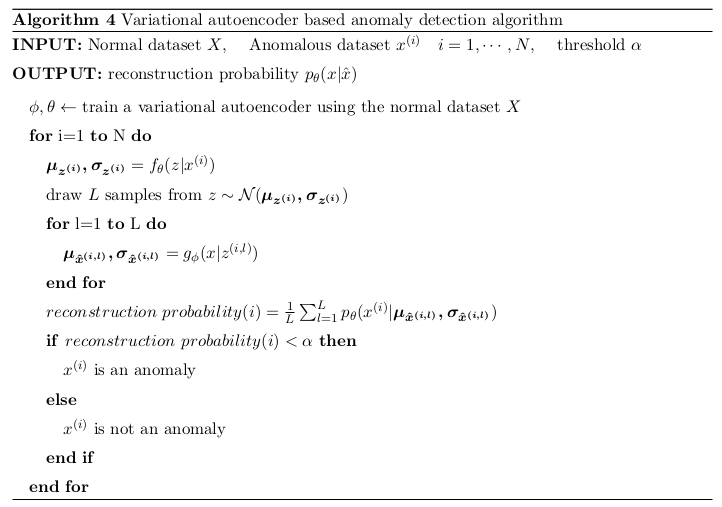
\includegraphics{img/2023-01-16-17-17-52.png}

The algorithm:

\begin{itemize}
\item
  VAEs learn a distribution of the inputs
\item
  The latent distribution \(p(z)\) acts as a prior (in Bayesian terms),
  and is the multivariate standard normal and isotropic (i.e.~separable,
  covariance matrix is diagonal)
\item
  \(f(x)\) is the encoder function
\item
  \(g(z)\) is the decoder function
\item
  The decoder function \(g(z)\) maps the distribution of the latent
  variable \(z\) into an output distribution \(p(x|z)\) which should
  resemble the original distribution of \(x\)
\item
  During reconstruction, when we sample a single latent variable \(z\),
  we reconstruct a single vector \(\hat{x}\), so we have a single sample
  of the output distribution \(p(x|z)\)
\item
  Idea for using Reconstruction Probability as an anomaly measure:

  \begin{itemize}
  \item
    sample multiple latent variables \(z^k\), and for each of them
    reconstruct the vector \(\hat{x}^k\)
  \item
    use all the vectors \(\hat{x}^k\) to estimate the probability
    \(p(x|z)\), and then compute the likelihood that the original input
    \(x\) comes from this distribution
  \item
    assuming \(p(x|z)\) is a an isotropic normal distribution, we just
    compute the mean \(\mu = E \lbrace \hat{x} \rbrace\) and covariance
    matrix \(\Sigma\) (diagonal, so basically we compute the variance
    \(\sigma_i^2\) per entry of the vector)
  \item
    the log-likelihood that the original \(x\) is generated by this
    distribution amounts to a weighted \(\ell_2\) norm:

    \[L(x) = \sum_i \frac{(x_i - \mu_i)^2}{\sigma_i^2}\]
  \item
    we use this as an anomaly score: small value = more anomaly, large
    value = more normal
  \item
    small value =\textgreater{} anomaly, because \(x\) does not fit the
    output probability \(p(x|z)\)
  \end{itemize}
\item
  Better than normal AE, because the variances are taken into account
\item
  Perhaps the variances \(\sigma_i^2\) can be used as indicators for
  feature selection?

  \begin{itemize}
  \tightlist
  \item
    or are they just similar to the clones values based on the input
    variances
  \end{itemize}
\end{itemize}

\hypertarget{wievel2019}{%
\subsubsection{Wievel2019}\label{wievel2019}}

\textbf{Continual Learning for Anomaly Detection with Variational
Autoencoder}

\begin{quote}
InProceedings (Wiewel2019)\\
Wiewel, F. \& Yang, B.\\
Continual Learning for Anomaly Detection with Variational Autoencoder\\
ICASSP 2019 - 2019 IEEE International Conference on Acoustics, Speech
and Signal Processing (ICASSP), 2019, 3837-3841
\end{quote}

\begin{itemize}
\item
  Use the full loss function as anomaly score, which includes the
  reconstruction error \textbf{and} the KL distance between the
  distribution of \(z\) and the standard normal prior \(p(z)\)

  \begin{itemize}
  \item
    \begin{quote}
    the so called evidence lower bound (ELBO):
    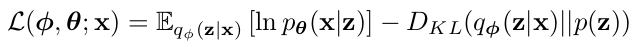
\includegraphics{img/2023-01-16-17-50-43.png}
    \end{quote}
  \item
    \begin{quote}
    While {[}4, 5, 6, 7{]} use the reconstruction probability E q φ
    (z\textbar x i ) {[}ln p θ (x i \textbar z){]} as the anomaly score,
    we use the ELBO as the anomaly score because it gives slightly
    better results in our experiments.
    \end{quote}
  \end{itemize}
\item
  The ``reconstruction probability'' used in An2015 is just the first
  part of the loss function (ELBO), why not use the full loss, since
  this is what the model was trained to minimize
\end{itemize}

\hypertarget{yao2023}{%
\subsubsection{Yao2023}\label{yao2023}}

\begin{quote}
Article (Yao2023)\\
Yao, Y.; Ma, J. \& Ye, Y.\\
Regularizing autoencoders with wavelet transform for sequence anomaly
detection\\
Pattern Recognition, 2023, 134, 109084
\end{quote}

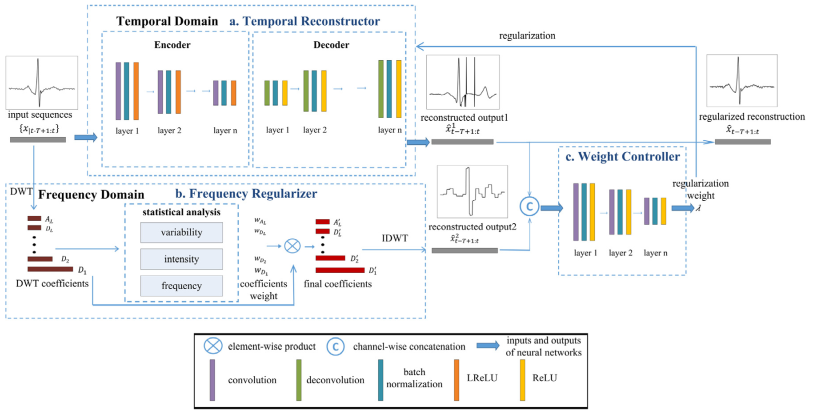
\includegraphics{img/2023-02-27-09-36-02.png}

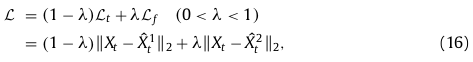
\includegraphics{img/2023-02-27-09-36-27.png}

\begin{itemize}
\tightlist
\item
  Use a custom loss function which includes filtering with DWT
\item
  Learn the regularization parameter \(\lambda\) which balances between
  AE loss and fixed DWT error
\item
  Only for training. In production, only AE used, as normal.
\item
  Empirical, non-reliable, DWT features
\item
  Idea: Learn \textbf{less} the vectors which are less modified by DWT

  \begin{itemize}
  \tightlist
  \item
    when second term is close to 0 (i.e.~input vector unchanged by DWT
    filtering), \(\lambda\) becomes close to 1, which reduces the
    influence of the AE loss, so the AE will learn \textbf{less} about
    these vectors
  \item
    so these vectors will be reconstructed more poorly, so more likely
    to be considered outliers
  \item
    a way to make some inputs more likely to be declared outliers:
    vectors untouched by DWT filtering are learned less, so more likely
    to be outliers
  \end{itemize}
\item
  Afterthoughts:

  \begin{itemize}
  \tightlist
  \item
    What if we \textbf{multiply} somehow two learnables?
    i.e.~\(\lambda \cdot \| AE loss \|\), or
    \(AE1 loss \cdot AE2 loss\). Which learns faster?
  \item
    If one NN learns first (e.g.~\(\lambda\)), it will reduce the
    incentive for the other one to learn.
  \item
    What if \(\lambda\) adapts much slower than the AE?
    \[(1 - \lambda) AE_{loss}  + \lambda Const\]
  \item
    AE loss drops first, then lambda will learn much later if the input
    is an outlier or not:

    \begin{itemize}
    \tightlist
    \item
      if AE loss is small, \(\lambda\) will be close to 1
    \item
      if AE loss is large, \(\lambda\) will be close to 0
    \item
      just an indirect reflection of AE loss / C ?
    \end{itemize}
  \item
    Two NNs in competition. Does it matter which one learns first?
  \item
    Outlier detection based on speed of learning?
  \end{itemize}
\end{itemize}

\hypertarget{lappas2021}{%
\subsubsection{Lappas2021}\label{lappas2021}}

\begin{quote}
InProceedings (Lappas2021)\\
Lappas, D.; Argyriou, V. \& Makris, D.\\
Fourier Transformation Autoencoders for Anomaly Detection\\
ICASSP 2021 - 2021 IEEE International Conference on Acoustics, Speech
and Signal Processing (ICASSP), 2021, 1475-1479
\end{quote}

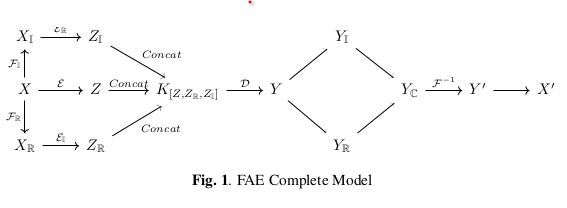
\includegraphics{img/2023-02-27-10-00-46.png}

\begin{itemize}
\tightlist
\item
  Augment input vector with Fourier transform, real and imaginary parts
\item
  Learn three coders, for each part
\item
  Concatenate the latent variables
\item
  A single decoder, which produces the real and imaginary parts
\item
  Architecture:

  \begin{itemize}
  \tightlist
  \item
    3N =\textgreater{} 3L =\textgreater{} 2N
  \end{itemize}
\item
  Y' to X' means what?? ``Another mapping''
\end{itemize}

\hypertarget{choi2023}{%
\subsubsection{Choi2023}\label{choi2023}}

\begin{quote}
TechReport (Choi2023)\\
Choi, J.; Park, J.; Japesh, A. \& Adarsh\\
A Subspace Projection Approach to Autoencoder-based Anomaly Detection\\
arXiv, arXiv, 2023
\end{quote}

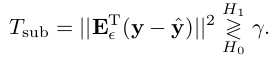
\includegraphics{img/2023-02-27-10-13-03.png}

\begin{itemize}
\tightlist
\item
  Information theoretic interpretation (MIMO), but not sure if useful at
  all
\item
  Practically: evaluate reconstruction error only on the subspace of the
  least significant eigenvectors of the error vectors

  \begin{itemize}
  \tightlist
  \item
    If error is large =\textgreater{} outlier, if small, normal
  \end{itemize}
\item
  \textbf{Just another example of weighted \(\ell_2\) norm}

  \begin{itemize}
  \tightlist
  \item
    here is in the space of the eigenvectors, inversely prop to variance
    (eigenvalues) (here just with 0, 1 binary selection)
  \item
    here it is the covariance matrix of all errors, since for AE we have
    a 1-to-1 input to output (single output vector)
  \item
    for VAE, we have the same idea, but the covariance matrix is per
    input vector, since we have 1-to-many (one input, multiple outputs)
    (see An2015)
  \end{itemize}
\end{itemize}



\end{document}
